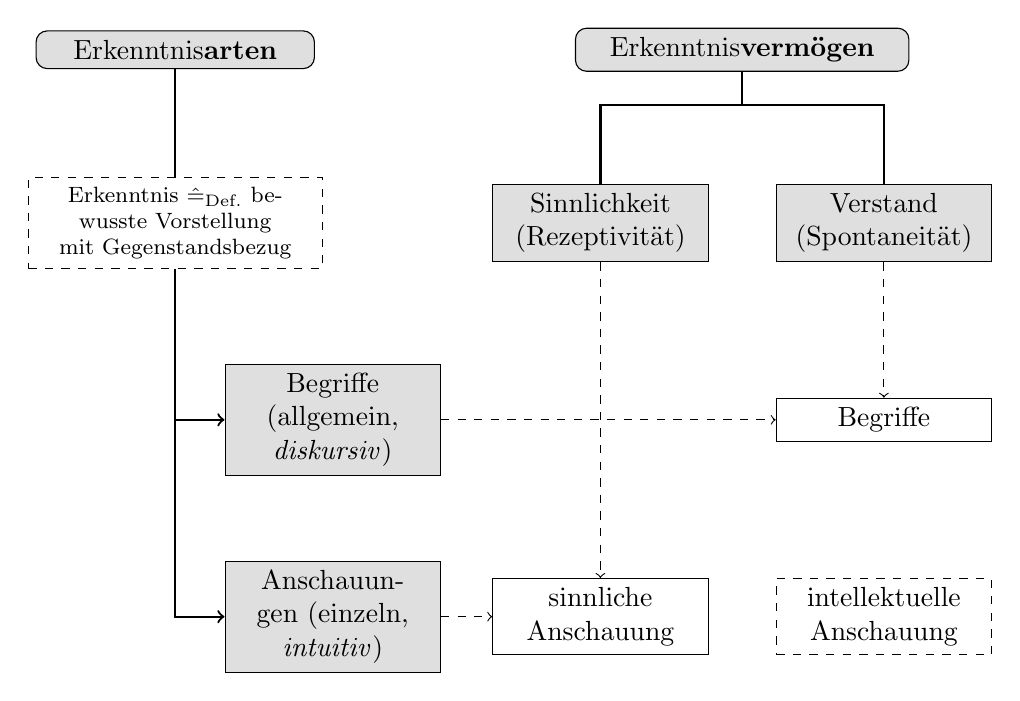
\begin{tikzpicture}%
[every node/.style={rectangle,draw=black,fill=gray!25, thin, text width=2.5cm,
align=center}]
\node (erkenntnisarten) at (0,7.2) [rounded corners, text
width=3.3cm] {Er\-kennt\-nis\-\textbf{ar\-ten}};
\node (erkenntnisvermoegen) at (7.2,7.2) [rounded corners, text width=4cm]
{Er\-kennt\-nis\-\textbf{ver\-mö\-gen}};
\node (defErk) at (0,5) [dashed, text width=3.5cm, font=\footnotesize,fill=none]
{Erkenntnis {\^=}\textsubscript{Def.} bewusste Vorstellung mit
Gegenstandsbezug}; \node (rezeptivitaet) at (5.4,5) {Sinnlichkeit (Rezeptivität)};
\node (spontaneitaet) at (9,5) {Verstand (Spontaneität)};
\node (begriffe) at (2,2.5) {Begriffe (allgemein, \emph{diskursiv})};
\node (beg) at (9,2.5) [fill=none] {Begriffe};
\node (anschauungen) at (2,0) {An\-schau\-un\-gen (einzeln, \emph{intuitiv})};
\node (sinnanschauung) at (5.4,0) [fill=none] {sinnliche Anschauung};
\node (intellAn) at (9,0) [fill=none, dashed] {intellektuelle Anschauung};
\draw [->,thick] (defErk.south) -- (0,2.5) -- (begriffe.west);
\draw [->,thick] (defErk.south) -- (0,0) -- (anschauungen.west);
\draw [-,thick] (erkenntnisvermoegen.south) -- (7.2,6.5) -- (5.4,6.5) --
(rezeptivitaet.north);
\draw [-,thick] (erkenntnisvermoegen.south) -- (7.2,6.5) -- (9,6.5) --
(spontaneitaet.north);
\draw [-,thick] (erkenntnisarten.south) -- (defErk.north);
\draw [->,dashed] (begriffe.east) to (beg.west);
\draw [->,dashed] (rezeptivitaet.south) to (sinnanschauung.north);
\draw [->,dashed] (spontaneitaet.south) to (beg.north);
\draw [->,dashed] (anschauungen.east) to (sinnanschauung.west);
\end{tikzpicture}
